\section{Análisis de los resultados}

En esta sección vamos a analizar los resultados obtenidos en la simulación, centrándonos principalmente en las diferentes contribuciones de cada fuente de incertidumbre a la anchura $\sigma$.  Vamos a usar la notación $\sigma(E^*)$ como anchura gaussiana a la distribución de energía de excitación reconstruida para $E^*$.  


\subsection{Reconstrucción sin fuentes d e incertidumbre}

En primer lugar vamos a analizar la reconstrucción de la energía de excitación sin considerar ninguna fuente de incertidumbre de las aquí modeladas. Como podemos ver en la imagen \cref{Fig:05-RecExcIdx3}, obtenemos prácticamente una distribución Breit-Wigner, con 

\begin{equation}
    \sigma_{0} (0) = \num{10.2(9.0)} \text{ keV} \quad 
    \sigma_{0} (0.2) = \num{2.8(2.5)} \text{ keV}
\end{equation} 
Uno de los posibles origenes de este término es que ROOT exija numéricamente un $\sigma$ real no nulo, para que la convolución voigt sea computable. También podría deberse a errores numéricos fruto del cálculo con números finitos. 

\vspace*{-0.25cm}
\begin{figure}[H]
    \centering
    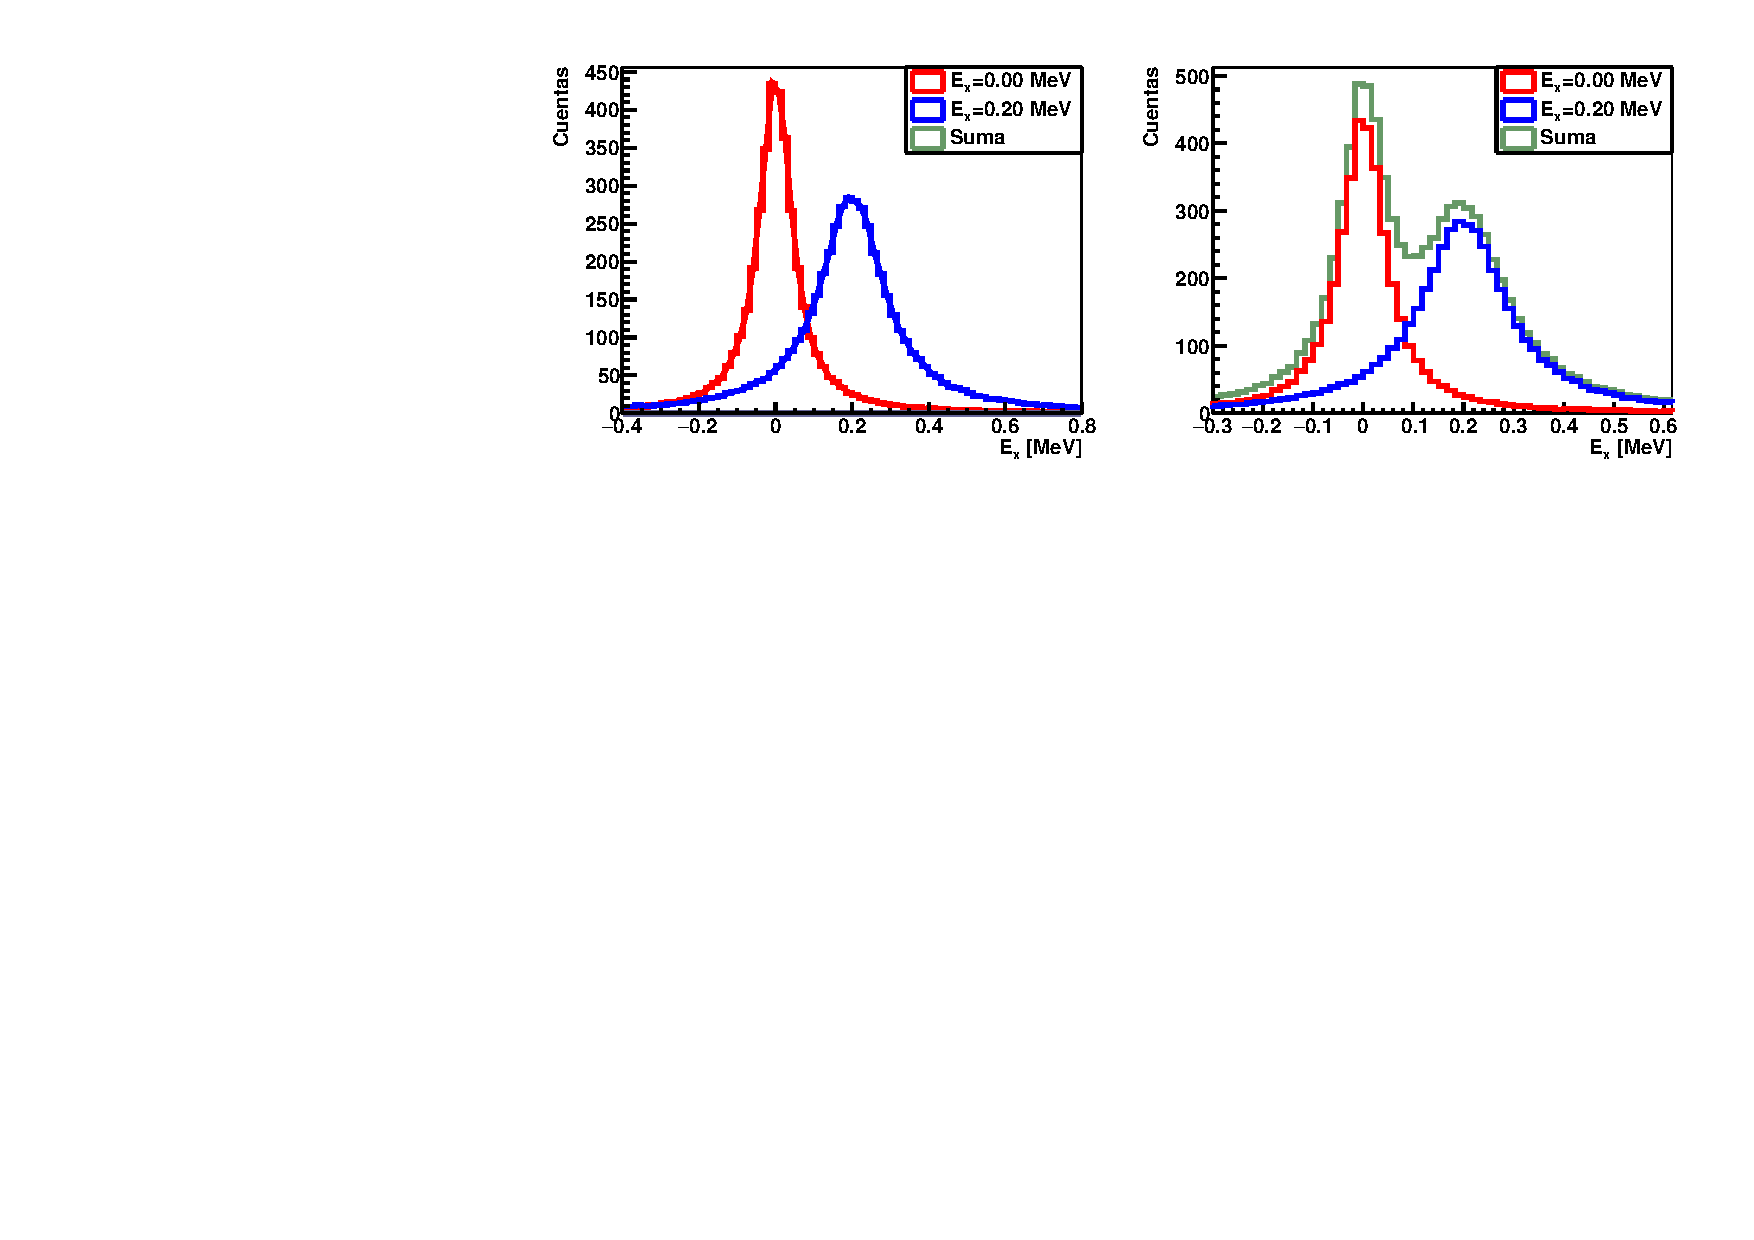
\includegraphics[width=0.95\textwidth]{Imagenes/Rec_incIdx3_single.pdf}
    \caption{$E_{ex}$ para $\sigma_{0}$. Izquierda, los espectros y ajuste Voigt. Derecha, los espectros y su suma.}
    \label{Fig:05-RecExcIdx3}
\end{figure}

\subsection{Reconstrucción solo con \textit{straggling}  y resolución del silicio}
95
En este apartado vamos a analizar la reconstrucción de la energía de excitación considerando únicamente el \textit{straggling} y la resolución del silicio, es decir, $\sigma_{straggling}$ y $\sigma_{sil}$, que se pueden considerar como
\begin{equation}
    \sigma_{str}^2 = \sigma_{straggling}^2 + \sigma_{sil}^2
\end{equation}
Como podemos ver en la imagen \cref{Fig:05-RecExcIdx1}, ahora ya vemos más superposición en los picos, tal que en la suma de ambos histogramas no diferenciamos dos picos como sí teníamos en el caso anterior. Curiosamente, es el efecto de la incertidumbre el que ahora hace que el pico más ancho sea el pico del estado fundamental y no del estado excitado. Todo esto se refleja en los resultados obtenidos: 

\begin{equation}
    \sigma_{str} (0) = \num{78.60(0.63)} \text{keV} \quad 
    \sigma_{str} (0.2) = \num{62.50(0.93)} \text{keV}
\end{equation} 

\begin{figure}[H]
    \centering
    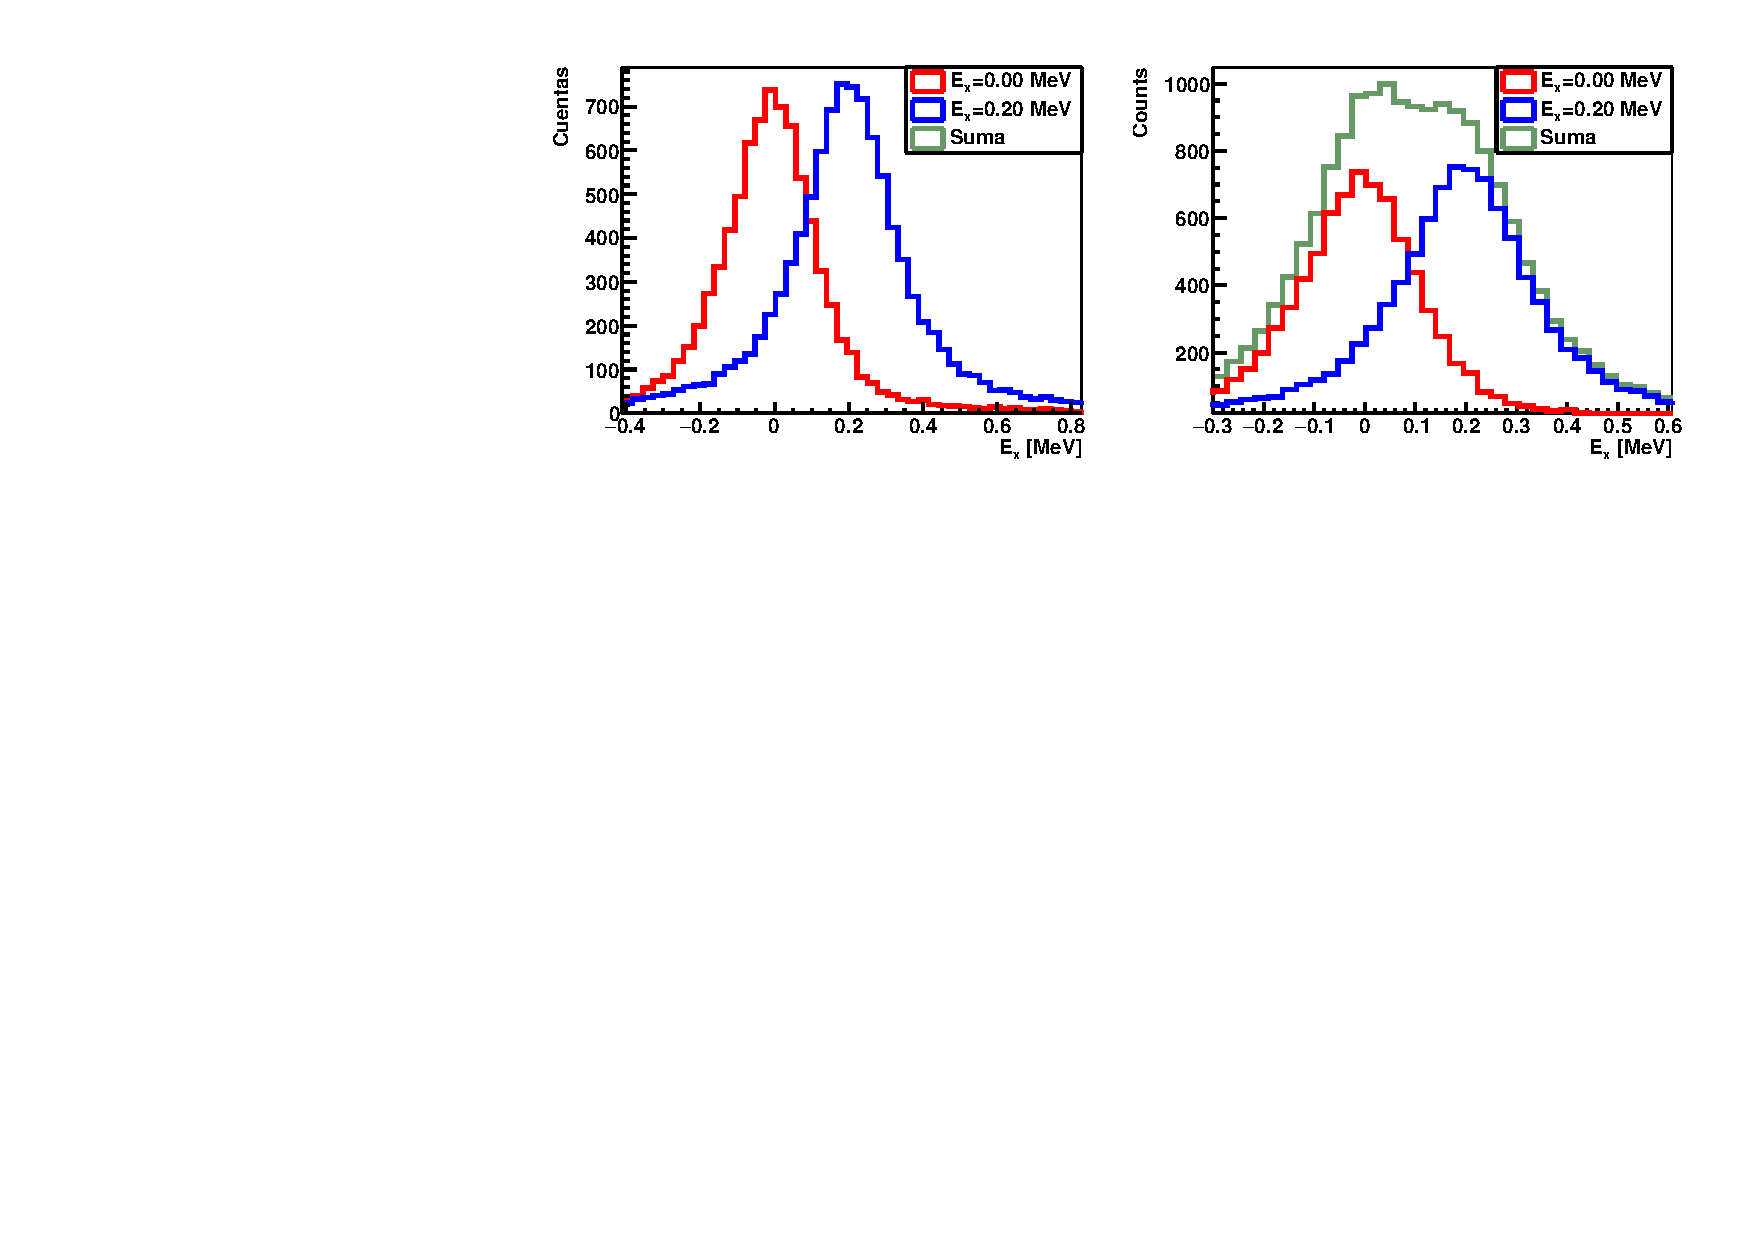
\includegraphics[width=0.95\textwidth]{Imagenes/Rec_incIdx1_single.pdf}
    \caption{$E_{ex}$ para $\sigma_{str}$. Izquierda, los espectros y ajuste Voigt. Derecha, los espectros y su suma.}
    \label{Fig:05-RecExcIdx1}
\end{figure}

\vspace*{-0.25cm}


En un principio el \textit{straggling}  debería contribuir por igual a ambos picos al tener una energía de excitación muy parecida y prácticamente el mismo rango. La diferencia radica en las secciones eficaces. Si nos fijamos en las secciones eficaces \cref{Fig:04-seccion_eficaz} y en la cinemática sampleada \cref{Fig:04-kinSampled0} y \cref{Fig:04-kinSampled2}, vamos claramente que para $E^*=0.0$ existe una mayor cantidad de estados con energías pequeñas, por lo que en realidad sufrirán más \textit{straggling} (en promedio) los tritios procedentes de interacciones en los que participa el estado fundamental. 


\vspace*{-0.45cm}
\subsection{Reconstrucción solo con resolución angular}

Aquí solo vamos a tener en cuenta el efecto de la dispersión angular, con el cual obtenemos una anchura gaussiana tal que: 

\begin{equation}
    \sigma_{\theta}(0.0) = \num{202.40(0.91)} \ \text{MeV} \quad 
    \sigma_{\theta}(0.2) = \num{171.3(1.0)} \ \text{MeV}
\end{equation} 
con un valor mucho más grande que el procedente de la interacción con la materia. En la imagen \cref{Fig:05-RecExcIdx2} podemos ver como ya no diferenciamos visualmente los picos en el histograma apilado. 

\vspace*{-0.25cm}
\begin{figure}[H]
    \centering
    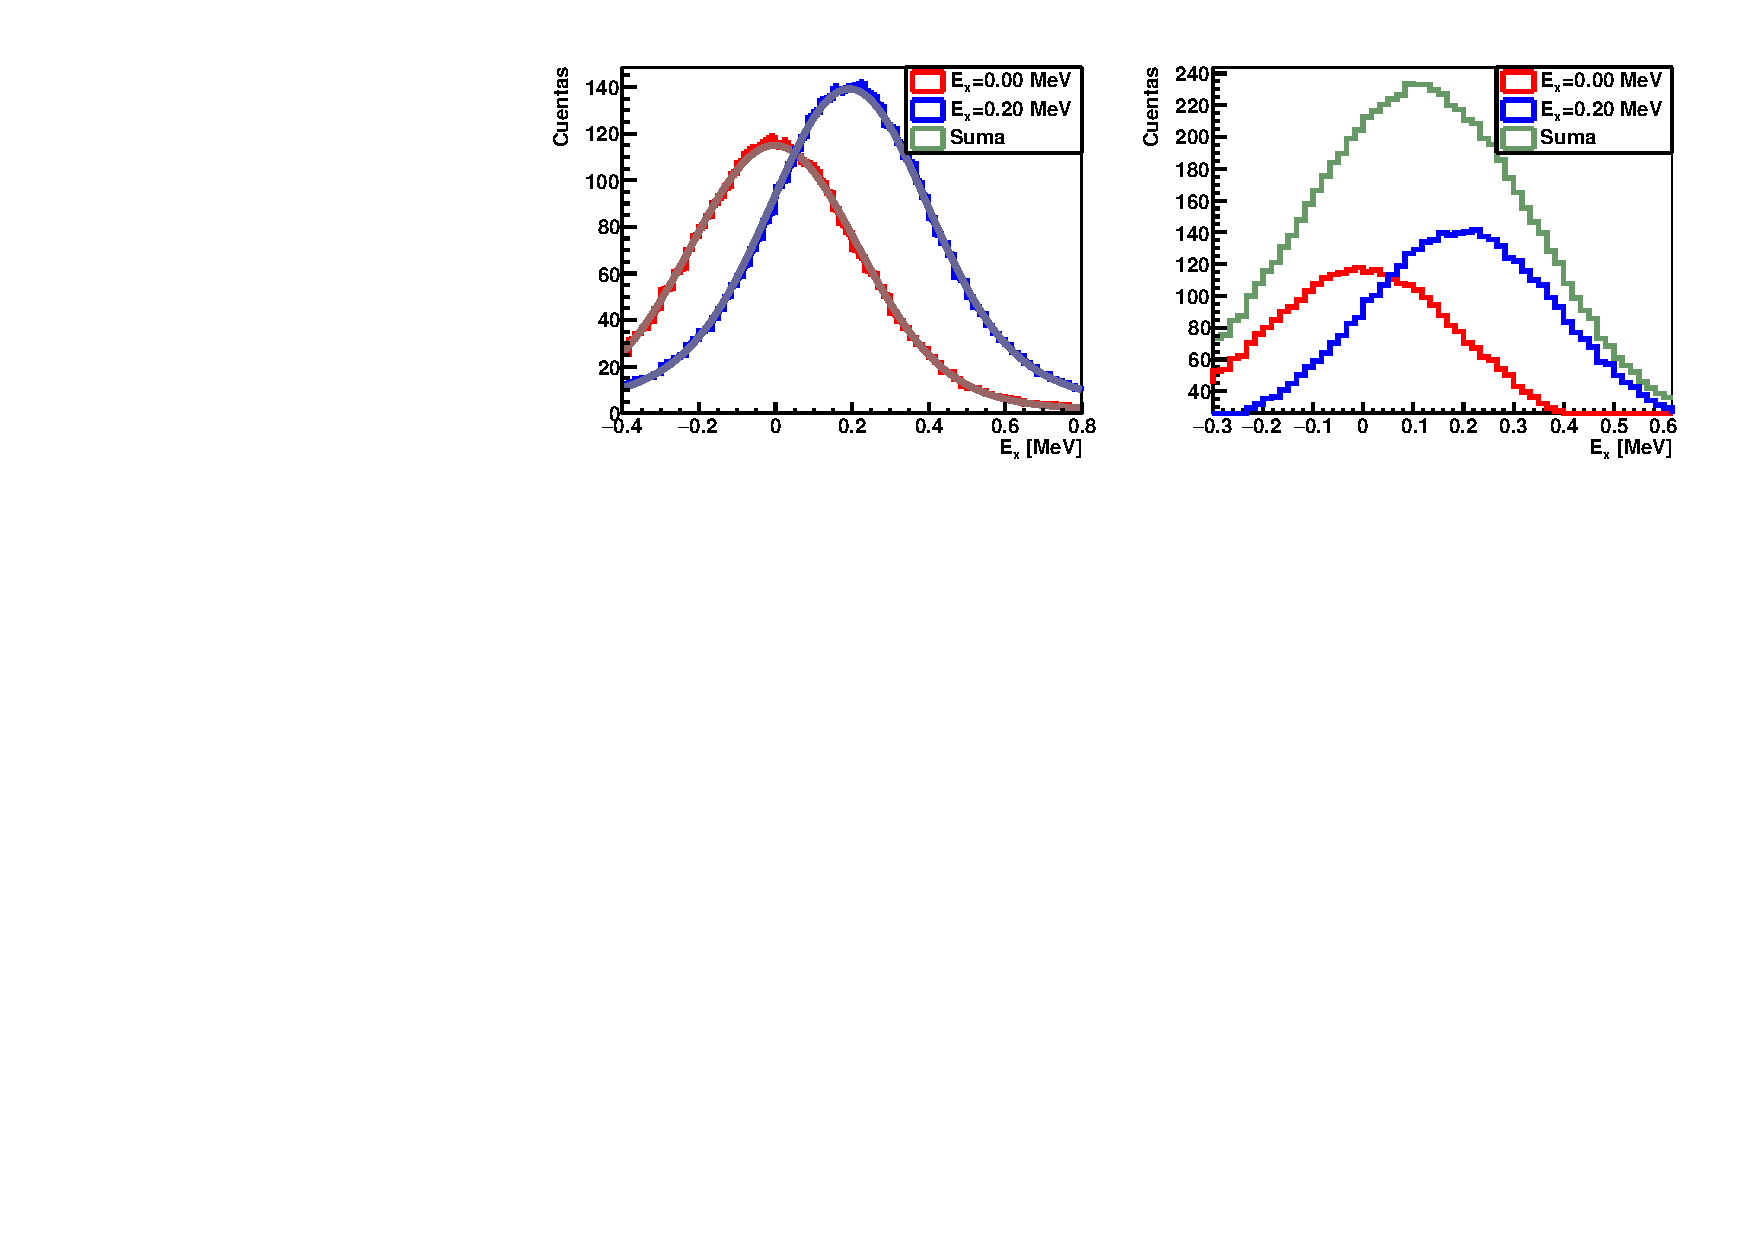
\includegraphics[width=0.95\textwidth]{Imagenes/Rec_incIdx2_single.pdf}
    \caption{$E_{ex}$ para $\sigma_{\theta}$. Izquierda, los espectros y ajuste Voigt. Derecha, los espectros y su suma.}
    \label{Fig:05-RecExcIdx2}
\end{figure}

\subsection{Reconstrucción con todas las fuentes de incertidumbre}

Aquí vamos a tener en cuenta todos las fuentes de incertidumbre implementadas, obteniendo así: 

\begin{equation}
    \sigma_{tot}(0.0) =\num{218.80(0.98)} \ \text{MeV} \quad 
    \sigma_{tot}(0.2) = \num{171.3(1.0)} \ \text{MeV}
\end{equation} 
e, igual que en el caso anterior, no podemos distiguir visualmente los picos del histograma apilado \cref{Fig:05-RecExcIdx0}. 

\begin{figure}[H]
    \centering
    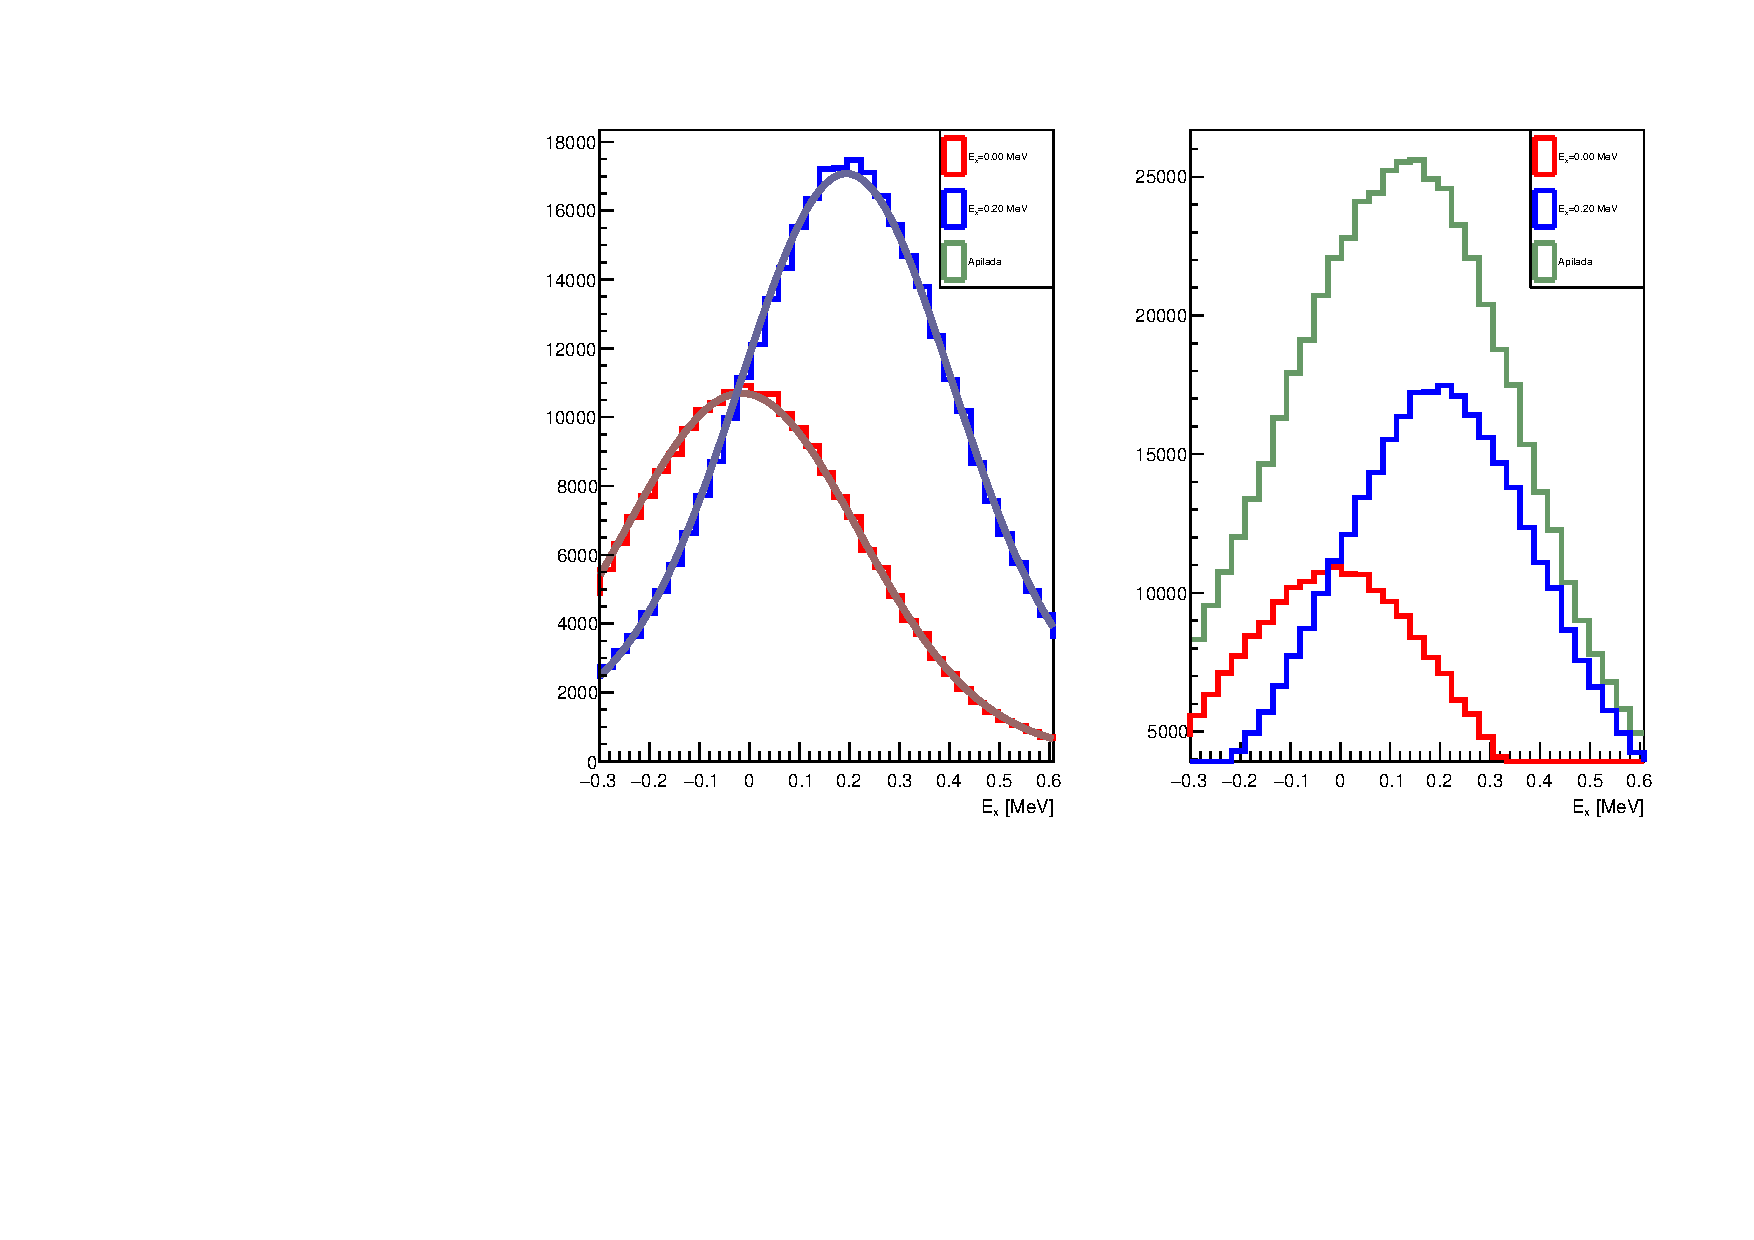
\includegraphics[width=0.95\textwidth]{Imagenes/Rec_incIdx0_single.pdf}
    \caption{$E_{ex}$ para $\sigma_{tot}$. Izquierda, los espectros y ajuste Voigt. Derecha, los espectros y su suma.}
    \label{Fig:05-RecExcIdx0}
\end{figure}


\subsection{Resumen de resultados}

En la \cref{Tab:05-ExcRec} mostramos los resultados de todas las $\sigma$ para las distribuciones gaussianas dentro de la función Voigt. Como podemos comprobar las $\sigma$ (y por tanto la FWHM)  si tenemos en cuenta todas las fuentes de incertidumbre y la anchura de la resonancia, de cada una de las distribuciones es mucho más grande que la distancia entre las energías del estado fundamental y el primer excitado. Para obtener un buen fit con el que poder obtener las energías de excitación tendríamos que ajustar las dos funciones Voigt con una sigma constante fijada, con los valores por ejemplo obtenido en esta simulación. La sigma aquí obtenida podría ser un parámetro constante que permitiría hacer el ajuste real y determinar las amplitudes $\Gamma$ en el experimento real. En la tabla \cref{Tab:05-GammaRec} podemos ver las anchuras $\Gamma$ que obtenemos con la reconstrucción, que en general es muy similar a los valores sampleados (de media un 5\% menor excepto para $\Gamma_0(0.2)$).  

\vspace*{2em}

\begin{minipage}{0.45\linewidth} \centering
\begin{tabular}{llll} \hline
\toprule 
 & $\sigma(0.0)$ [MeV]  &  $\sigma(0.20)$ [MeV]  \\ \midrule 
$\sigma_{tot}$ & $\num{0.221399220037(0.0021212987)}$ & $\num{0.185196321591(0.0022299371)}$\\ 
$\sigma_{straggling}$ & $\num{0.089228019253(0.0014396243)}$ & $\num{0.066717598649(0.0020985552)}$\\ 
$\sigma_{\theta}$ & $\num{0.202223846486(0.0020712731)}$ & $\num{0.173000700171(0.0022192850)}$\\ 
$\sigma_{0}$ & $\num{0.012904479318(0.0023798058)}$ & $\num{0.018380035441(0.0040286966)}$\\ 
 \bottomrule 
\end{tabular}

\captionof{table}{$\sigma$ del ajuste voigt a la distribución de energía de excitación reconstruida.}
\label{Tab:05-ExcRec}
\end{minipage}
\hfill
\begin{minipage}{0.45\linewidth} \centering
\begin{tabular}{llll} \hline
\toprule 
 & $\Gamma(0.0)$ [keV]  &  $\Gamma(0.20)$ [keV]  \\ \midrule 
$\Gamma_{tot}$ & $\num{96.0(1.4)}$ & $\num{194.2(1.4)}$\\ 
$\Gamma_{str}$ & $\num{99.7(0.93)}$ & $\num{197.2(1.0)}$\\ 
$\Gamma_{\theta}$ & $\num{98.0(1.3)}$ & $\num{195.9(1.4)}$\\ 
$\Gamma_{0}$ & $\num{97.3(0.95)}$ & $\num{177.1(0.81)}$\\ 
 \bottomrule 
\end{tabular}

\captionof{table}{$\Gamma$ del ajuste voigt a la distribución de energía de excitación reconstruida.}
\label{Tab:05-GammaRec}
\end{minipage}

\vspace*{2em}